
\section{Results / Assessment}

As the MC estimates, used to approximate the gradient of the likelihood are based on random samples of the model distribution and the data distribution respectively,
are themselves random variables, the entire estimation process is stochastic in nature and we can view it as a stochastic process.

Since the sequence of parameter estimates at every iteration is essentially a realisation of this stochastic process, the error metrics can be viewed as one as well.
Suppose for an experiment a full training procedure is conducted with a total number of $n$ iterations across epochs.
Because of the stochastic nature of the training the training procedure is repeated $m$ times, with the same hyper parameters, 
to get an impression of the parameter estimation process as a whole.
For any error metric $M$ we then obtain a set of $m$ time series of length $n$ and can write $M_i (j)$ for the value of the metric for training run $i$ at iteration $j$.
So the comparisons in the following are done by assessing and plotting the development of the error measures or likelihood values as stochastic processes,
and by their final parameter estimate.


\subsection{Remarks on Hyperparameters}

Assessing performance of learning in this context is complicated a lot by the large number of hyperparameters 
and the fact that the best choice of these is typically model dependent.
In order to simplify the task and level the playing field some are thus chosen as fixed.
In all experiments the used optimiser is ADAM \cite{Kingma2014AdamAM} and the learning rate is fixed to $\alpha = 10^{-3}$ as recommended in the paper.
In ADAM $\alpha$ is used in form of a coefficient in front of a linearly transformed form of the gradient
\[
	\bm{\theta}_{k+1} = \bm{\theta}_k - \alpha f( \nabla_{\bm{\theta}} \text{NLL}(\bm{\theta}_k) )
\]

and as the framework uses the MC estimates directly the gradient is $\frac{1}{b} \nabla_{\bm{\theta}} \text{NLL}(\bm{\theta}_k)$, 
and thus the de-facto learning rate changes with the batch size, from $\alpha$ to something like $\frac{\alpha}{b}$.
The batch size is also set fixed to $b = 200$ samples per batch so the learning rate is set at $\alpha = \frac{200}{10^{-3}} = 0.2$
This learning rate may not be the optimal choice for any of the tested models, but makes comparisons easier and more direct.

The number of epochs is set to $10$ and with a randomly loaded dataset of $10^4$ samples.
Thus the resulting total number of training iterations for a complete training run is $n = 500$.
All samplers require a starting batch which is set to zeros.
Excepted when claimed otherwise all experiments have been run repeating the training procedure $m = 50$ times.
Thus when talking about a mean for an experiment setting this mean is taken across training procedures.
The parameter process plots shown later represent the mean and standard deviation of the parameter process, 
where the estimates at each training iteration are averaged across training runs, i.e. for a metric $M$ 
\[
	M (j) = \frac{1}{m}\sum_{i=1}^m M_i(\bm{\theta} - \hat{\bm{\theta}}_j )
\]

\subsection{The Choice of the Sampler Step Size}

The choice of the sampling step size $\varepsilon$ is a complex problem.
In many experiments the estimation process broke down due to the choice of $\varepsilon$.
This was due to two main problems:

For the polynomial model, as stated before, ULA sampler is inherently unstable and even during a single training step the sampling process can diverge easily.
It is a distribution with very light tails and the probability mass is concentrated in a small region.
If a sample in just one of the chains happens to be close to the boundary of the complement of that region, in which the energy increases very strongly,
then a random step can take it to a location where the state has very large energy.
This in turn produces a very large gradient in absolute value, and that gradient can push the chain in the opposite direction such that it again lands in a region of high energy.
Essentially this chain then fluctuates itself to infinity, which breaks the parameter gradient, leading to a breakdown of the training.

This does not happen for ULA and MALA due to their acceptance step, but there is still a problem with the instability of the models.
\texttt{pytorch} has no direct mechanism to constrain parameters to a specific domain, and so the models discussed here can have their parameters changed in such a way,
that they are no longer probability distributions, which subsequently leads to a breakdown of the training procedure.
For the polynomial model, the coefficient of the highest order monomial needs to be positive, otherwise the density simply turns into an exploding exponential function.
Something similar happens in the Gaussian models.
If any of the covariance matrices stop being positive semi-definite the energy can turn negative and the same problem of an unbounded density occurs.
This problem is especially pronounced in the beginning of the training procedure and depends both on $\varepsilon$ and the start batch.
The start batch was set to zeros, both for convenience and to reflect the issue that a good start batch from the model distribution is unavailable for complex models.
But of course a batch of zeros does not represent the model distribution and if the burnin or $\varepsilon$ are too low,
then the samples generated initially from the start batch poorly reflect the model distribution and 
effect large parameter gradients that can push the parameters to infeasible regions in the first couple training iterations.

One could counteract this problem by reducing the learning rate but here the approach was to adapt the step size $\varepsilon$ instead for consistency.
Both for MALA and HMC a larger step size like $\varepsilon = 10^{-1}$ turned out to be mostly stable.
For ULA this was also true for the Gaussian models but not for the polynomial where the problem described first led to divergence.

\subsection{Expectations}
As the recovery adaptation makes the distribution to be sampled from more unimodal the smaller the perturbation variance is chosen,
one can expect RL to do better the more multimodal the target and starting distribution are.
There should be a tradeoff between burnin choice and quality of the estimates.
Burnin has the largest impact on overall training time.
This is intuitively easy to understand as every sampling process involves iterating as many chains as the batch dimension $\text{burnin} +1$ times.
With a high burnin both ML and RL can be expected to perform similarly well.
The higher the burnin the closer the samples are to the model distribution in ML, so a higher burnin can be expected to improve quality overall.
This improvement comes at the cost of training iteration time however, which is the essential conundrum that RL intends to resolve.
Thus the main focus of testing for RL here is to compare the results when the burnin is set low, 
as even with relatively low burnin the resulting samples at each iteration should be more accurate when the original distribution is multimodal.

RL does have an additional price during every sampler iteration, 
which comes from calculating the conditional components at every call to the \texttt{energy} and \texttt{energy\_grad} methods during sampling.
Additionally the samples that the methods are conditioned on have to be reset after each training iteration.
If the distribution is itself unimodal this should be a price without extra gain, but when the distribution is otherwise difficult to sample from,
then RL could allow to use a lower burnin.


\subsection{Univariate Polynomial}

The polynomial model was tested with a bimodal target distribution with target parameters:
\[
\begin{aligned}
	\bm{w} &= (w_1, w_2, w_3, w_4) = ( -1.2, -0.7, 2, 1 ) \\
	&\text{i.e.} \\
	U(x) &= x^4 + 2 x^3 - 0.7 x^2 - 1.2 x \\
\end{aligned}
\]
and an unimodal start distribution with the parameters:
\[
\begin{aligned}
	\bm{w}_0 &= (w_1^0, w_2^0, w_3^0, w_4^0) = ( 1, 1, 1, 1 ) \\
	&\text{i.e.} \\
	U_{\bm{w}_0} (x) &= x^4 + x^3 + x^2 + x \\
\end{aligned}
\]

\begin{comment}
\begin{figure}[H]
  	\centering
  	\includegraphics[width=0.75\linewidth]{assets/data_vis/Bimodal_Maj_Unimodal_Min.png}
  	\captionof{figure}{Target and start density}
  	\label{fig:Mode_Experiment}
\end{figure}
\end{comment}
As the model is one dimensional in the input it is fairly fast to train and was tested most comprehensively.
For MALA and HMC the step size was set to $\varepsilon = 10^{-1}$, 
but for ULA sampler consistently diverged for this setting so all tests for ULA were done with $\varepsilon = 10^{-2}$.
This may seem like an unfair comparison as a higher step size allows for faster convergence, if convergence happens at all.
But this disadvantage for ULA is somewhat mitigated by the fact that the sample distribution for both MALA and HMC tend to change much slower overall
due to the acceptance step, which causes chains of both samplers to often remain in a state for some time in the onset of the training process.

A full training procedure was run for all combinations of the samplers and the following settings for burnin and perturbation variance
\begin{enumerate}
	\item Burnin $\in [10, 20, 50, 100]$
	\item Perturbation variance $\sigma \in [0.1, 0.5, 1]$
\end{enumerate}

for RL and without the perturbation variance also for ML. This resulted in a total number of more than a million training iterations combined.

In most of the conducted experiments ML performed better across the board, but in some settings RL obtained better results on average.
One important result was that the choice of perturbation variance is extremely important for RL.
Choosing $\sigma = 0.1$ produced parameter divergence irrespective of the sampler used.
\begin{figure}[H]
  	\centering
  	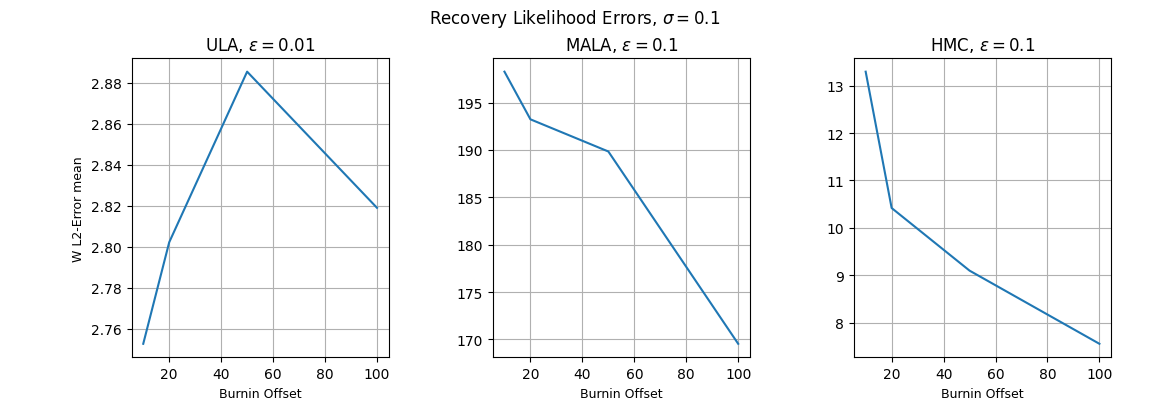
\includegraphics[width=0.85\linewidth]{assets/figures/low_sigma_recov.png}
  	\captionof{figure}{Recovery Likelihood error for $\sigma = 0.1$ against burnin}
  	%\label{fig:Mode_Experiment}
\end{figure}

In that setting, while still performing very poorly, ULA surprisingly performed the best. 
A reason for this could be that the data samples upon which the recovery adapter conditions change at every training iteration.
If $\sigma$ is too small, and the conditional distribution has thus low variance, then changing the samples can potentially shift the mean 
and effectively reset the convergence of the chains. 
Especially for MALA and HMC this could lead to a large number of rejected samples and thus poor sample quality, 
where the chains might remain mostly in their previous modes.

As the parameters diverged for $\sigma = 0.1$ these runs are excluded in the following results.


\subsubsection{Results for ULA}

For larger burnin, recovery likelihood with $\sigma = 0.5$ actually outperformed ML, with both better final errors and a lower standard deviation.
\begin{figure}[H]
  	\centering
  	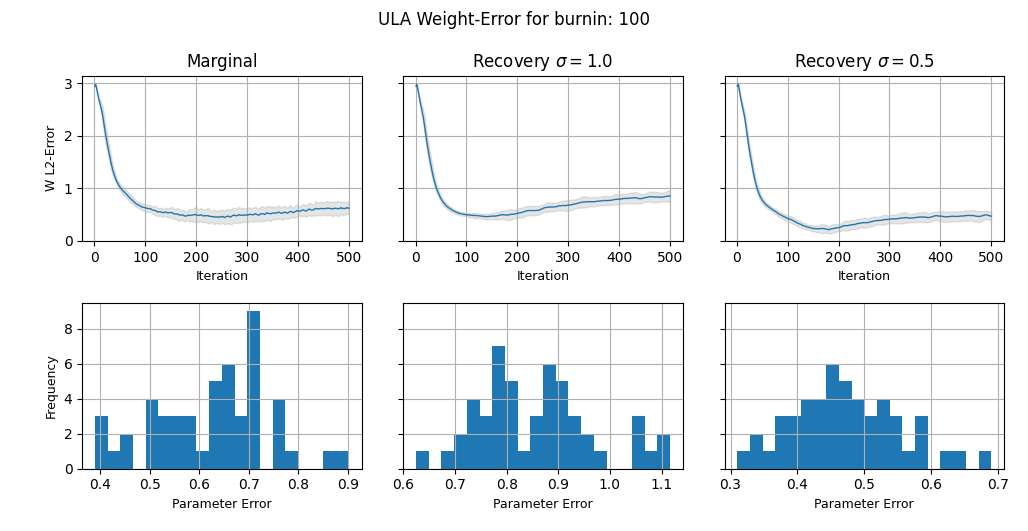
\includegraphics[width=0.85\linewidth]{assets/figures/POLY_ULA_burnin100.png}
  	\captionof{figure}{
		ULA performance across runs. 
		The upper plots represent the entire parameter process, histograms show final error
	}
  	%\label{fig:Mode_Experiment}
\end{figure}

The average error for ML at this setting was at $0.62$ with a standard deviation of $0.11$, 
while RL had an average error of $0.47$ with a standard deviation of $0.08$.
This trend reversed rapidly when decreasing the burnin however, with noticeably worse results for both settings of RL at a burnin lower than $50$.
\begin{figure}[H]
  	\centering
  	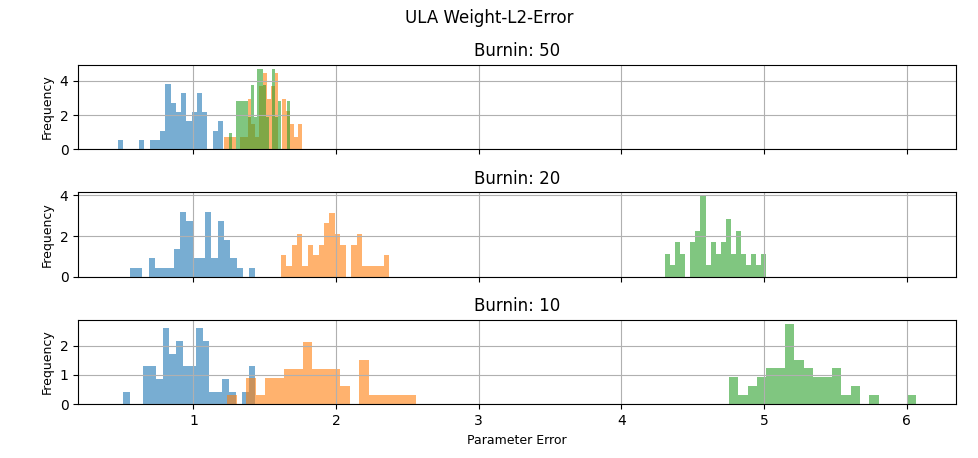
\includegraphics[width=0.85\linewidth]{assets/figures/POLY_ULA_burnins.png}
  	\captionof{figure}{
		ULA performance across runs. 
		Marginal Likelihood (blue), RL with $\sigma = 0.5$ (green), RL with $\sigma = 1.0$ (orange)
	}
  	%\label{fig:Mode_Experiment}
\end{figure}

It is noteworthy that ML didn't suffer as significantly as expected for the lower burnins, although the overall performance was worse using ULA.


\subsubsection{Results for MALA}

The experiments with MALA show a trend for the variance of the RL estimator more clearly.
For a burnin of $100$ the overall estimates are fairly good, but we can see that decreasing $\sigma$ increases the variance of the final estimator.

\begin{figure}[H]
  	\centering
  	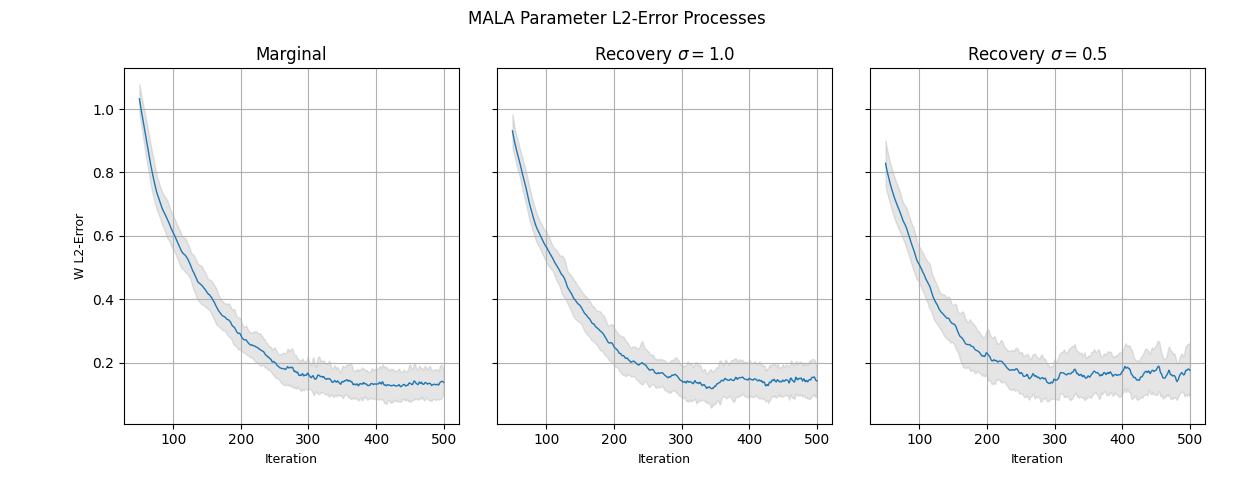
\includegraphics[width=0.85\linewidth]{assets/figures/POLY_MALA_pro100.png}
  	\captionof{figure}{
		MALA processes for burnin $100$.
		RL for $\sigma = 0.5$ shows significantly higher variance
	}
  	%\label{fig:Mode_Experiment}
\end{figure}






\subsection{Multivariate Gaussian Model}

The multivariate Gaussian distribution is unimodal and easy to sample from. 
It serves as a baseline, for which one would expect both ML and RL do perform similarly well in terms of estimate quality.
The test model is two dimensional with target parameters
\[
\begin{aligned}
	\mu &= \begin{pmatrix} 3 \\ 3 \end{pmatrix} \\
	\Sigma &= 
	\begin{pmatrix}
		2 & 0 \\
		0 & 2 \\
	\end{pmatrix} \\
\end{aligned}
\]

and start parameters
\[
\begin{aligned}
	\mu_0 &= \begin{pmatrix} 2 \\ 2 \end{pmatrix} \\
	\Sigma_0 &= 
	\begin{pmatrix}
		2 & 0 \\
		0 & 1 \\
	\end{pmatrix}. \\
\end{aligned}
\]


\subsection{Gaussian Mixture Model}
Target parameters:
\[
\begin{aligned}
	&\mu_1 = \begin{pmatrix} 2 \\ 2 \end{pmatrix}  &\hspace{20pt}  &\mu_2 = \begin{pmatrix} -1 \\ -1 \end{pmatrix} \\
	&\Sigma_1 = 
	\begin{pmatrix}
		2 & 0 \\
		0 & 2 \\
	\end{pmatrix} 
	&\hspace{20pt}
	&\Sigma_2 = 
	\begin{pmatrix}
		1 & 0 \\
		0 & 1 \\
	\end{pmatrix} \\
\end{aligned}
\]
with weights $(w_1, w_2) = ( 0.2, 0.8 )$

Start parameters:
\[
\begin{aligned}
	&\mu_1^0 = \begin{pmatrix} 3 \\ 3 \end{pmatrix}  &\hspace{20pt}  &\mu_2^0 = \begin{pmatrix} 1 \\ 0 \end{pmatrix} \\
	&\Sigma_1^0 = 
	\begin{pmatrix}
		3 & 0 \\
		0 & 1 \\
	\end{pmatrix} 
	&\hspace{20pt}
	&\Sigma_2^0 = 
	\begin{pmatrix}
		2 & 0 \\
		0 & 2 \\
	\end{pmatrix} \\
\end{aligned}
\]
with weights $(w_1, w_2) = ( 0.5, 0.5 )$





\begin{comment}


\begin{table}[H]
\centering
%\csvautotabular{assets/tables/distance_mean_values.csv}
\csvreader[
	tabular = *{6}{|c}|,
	table head = \hline \bfseries {cluster distance} & \bfseries accuracy & \bfseries precision & \bfseries  recall & \bfseries {F1-score} & \bfseries {ROC AUC Score}\\\hline, 
	late after line = \\\hline
	]{assets/tables/distance_mean_values.csv}{}{%
	\csvcoli & \csvcolii & \csvcoliii & \csvcoliv & \csvcolv  & \csvcolvi
}
\caption{Table aggregated by cluster distance}
\end{table}

%----------------------------------------------------------------------------------------------------------------------------------------------------------------------------------------------------
\subsection{Univariate Polynomial}
ULA epsilon = 1e-1 -> NaN cascade
ULA epsilon = 1e-4 -> NaN cascade

%----------------------------------------------------------------------------------------------------------------------------------------------------------------------------------------------------
While there is a lot of theory developed for stochastic processes, 
the complexity contributed by the components of the learning procedure makes it very hard to derive the parameter process analytically.
Even assuming that the samplers for the model provide bona fide samples of the model distribution, 
the randomness of the model samples and of the batch selection comes in in the form of gradients of the likelihood.
It is then warped by the optimisation procedure, which could itself be stochastic algorithm.


Hence there are a lot of dependencies and the evaluation here is empirical and, due to the vast space of hyper parameters and potential choices in strategy,
necessarily not comprehensive.


%----------------------------------------------------------------------------------------------------------------------------------------------------------------------------------------------------
\subsection{Effect of the Sampler-Stepsize} 

The more we decrease $\varepsilon$ the smaller the steps we take in the sampler iterations.
One effect is that it is more likely to get stuck in a vast mode, depending on the distribution.
Another effect is that we decrease the contribution of the gradient compared to the contribution of the random fluctuations.
This is because the square root makes values significantly larger the closer $x$ is to 0.
When considering the stochastic process, which we discretise, this makes intuitive sense.
The more we zoom into the graph of a realisation of an Ito process, the less 'visible' the effect of the drift term becomes, 
and the more pronounced one can observe the erratic behaviour of the Wiener process term.

Suppose we have a distribution with very light tails and that the probability mass is concentrated in a small region, like the one induced by the polynomial energy, 
and that our chain happens to be close to the boundary of the complement of that region in which the energy increases very strongly.
If we choose a large step size the gradient dominates and the steps are big, potentially overcorrecting and moving the chain into a region with very high energy.
But if we choose the step size too low, the stochastic term dominates and can randomly push the chain into a region with very high energy again.
Intuitively this is the reason why the ULA sampler can easily diverge, both for too large and too low step sizes.
\end{comment}













